\chapter{Problem Analysis \& Solution}

Present the solution.

\begin{itemize}
\item Mention related works
\item Describe the main idea behind the clustering techniques used
\item Describe the main idea behind the various visualizations
\end{itemize}

More in detail:

\begin{itemize}
\item The main trick is to convert a mesh difference visualization problem to a vector field visualization problem. The methods developed there are very good and can be applied in our case. Talk about the research done for clustering.
\item Used methods were chosen because of their simplicity. In case they had proven insufficient, it would have been possible to replace them easily by a more sophisticated version as clustering only constitutes one part of the visualization process.
\item Now describe the solution.
\end{itemize}

%%-----------------------------------------------------------------------------------------
%%-----------------------------------------------------------------------------------------
\section{Seeing Mesh Difference as a Vector Field}

In our new visualizations, arrows will be used to represent the difference between two triangle meshes. Each arrow will be internally represented by a position and a direction vector. Together, they will form a discrete and bounded vector field. This is a very important abstraction because vector field visualization is a very rich area which finds applications in engineering, molecular modeling and computational fluid dynamics. Therefore, there exist many scientific papers studying this topic, such as \citet{Telea99}, \citet{Garcke00}, \citet{Du04} or \citet{Peng12}.

When visualizing a vector field, it is necessary to use clustering on the vectors to obtain a simplified representation, otherwise the visualization becomes too cluttered (see fig. \ref{fig:meshdiff_unclustered}). Clustering therefore determines to a large extent what the final visualization will look like.

\begin{figure}[h]
\centering
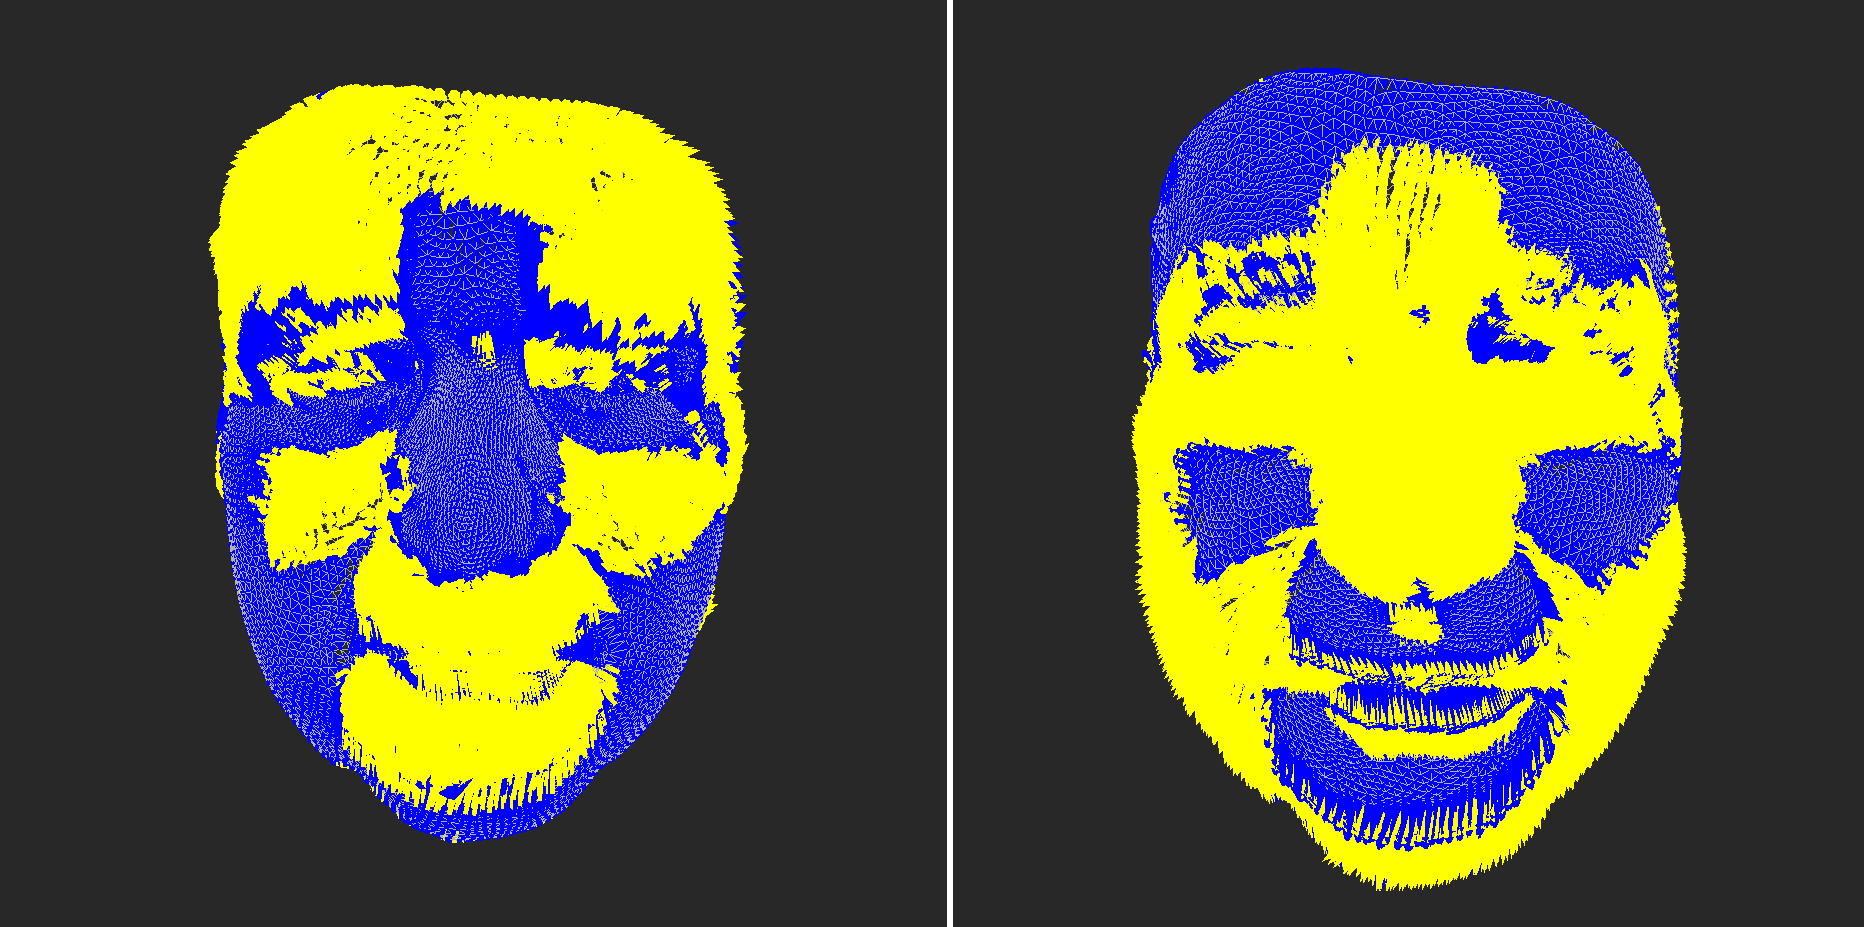
\includegraphics[width=\textwidth]{./img/meshdiff-unclustered_arrows.PNG}
\caption{MeshDiff - Vertex distance visualized by unclustered arrows}
\label{fig:meshdiff_unclustered}
\end{figure}
%%-----------------------------------------------------------------------------------------
%%-----------------------------------------------------------------------------------------
\section{Arrow Clustering}


%%-----------------------------------------------------------------------------------------
%%-----------------------------------------------------------------------------------------
\section{Proposed Visualizations}